\newpage
\section{Описание пользовательского интерфейса}

Пользовательский интерфейс инструмента представляет собой главное окно, в котором пользователь может создавать вкладки (как в браузере).
В каждой вкладке может происходить редактирование различных исходных текстов баз знаний представленных с помощью различных языков. 
По сути каждая вкладка - это некоторый редактор исходных текстов представленных на некотором внешнем языке. К примеру, это может быть 
редактор sc.g-текстов, редактор sc.n-текстов, редактор sc.s-текстов и т. д.
Набор возможных редакторов определяется набором установленных расширений.

В рамках главного окна имеется панель инструментов, и меню приложения. Меню приложения представляет собой некоторый набор команд. 
Команды, которые отображаются в меню делятся на два типа:
\begin{list}{•}{}
	\item команды, которые являются общими для всех вкладок. В частности к ним относятся команды сохранения, загрузки, помощи и т. д.
	\item команды, которые специфичны для активной вкладки. Зависят от типа активной вкладки.
\end{list}

На панель инструментов, как и в пользовательских интерфейсах большинства приложений, вынесены наиболее часто используемые команды:
\begin{list}{•}{}
	\item \textbf{Создать новый файл} - отображает диалог, в котором пользователю предлагается выбрать формат нового файла.
	Для выбранного пользователем формата создается новая вкладка. Список возможных форматов определяется набором установленных расширений:
	
	\begin{figure}[h]
		\begin{center}
			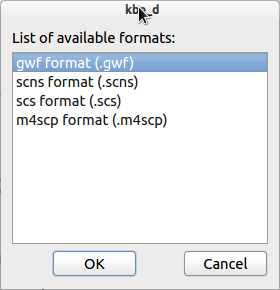
\includegraphics[scale=0.7]{../images/new_dialog.png}
		\end{center}
		\caption{Диалог выбора формата}
		\label{pic_new_dialog}
	\end{figure}
	
	
	\item \textbf{Открыть файл} - открывает диалог выбора файла. Выбранный файл открывается в новой вкладке.
	\item \textbf{Сохранить} - сохраняет содержимое активной вкладки в файл. При этом если содержимое вкладки 
	уже было сохранено в файл или же оно было заргужено из файла, то сохранение будет выполнено именно в этот файл (путь к нему указан в имени вкладки).
	В противном случае поеведение этой команды будет эквивалентно команде \textbf{Сохранить как}
	\item \textbf{Сохранить как} - открывает диалог выбора файла. Содержимое активной вкладки созраняется в выбранный файл.
	\item \textbf{Закрыть} - закртывает активную вкладку. Если в ней имеются не сохраненные даные, то отображается диалог уточняющий необходимость
	их сохранения.
\end{list}

Каким образом выглядит главное окно, можно увидеть на следующем рисунке:
\begin{figure}[h]
	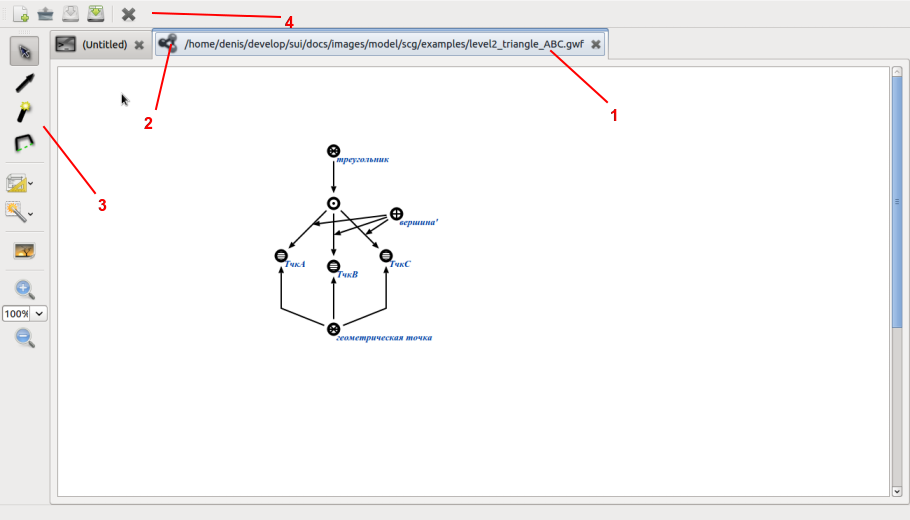
\includegraphics[width=16.23cm, height=9.82cm]{../images/tabs.png}
	\caption{Вкладки в рамках главного окна приложения. 1 - имя вкладки (путь к редактируемому файлу), 2 - иконка, которая показывает
	тип редактируемого текста внутри вкладки, 3 - панель, которая относится к активной вкладке, 4 - основная панель инструментов главного окна}
	\label{pic_tabs}
\end{figure}

%\subsection{Главное окно приложения}
%\begin{figure}[h]
%	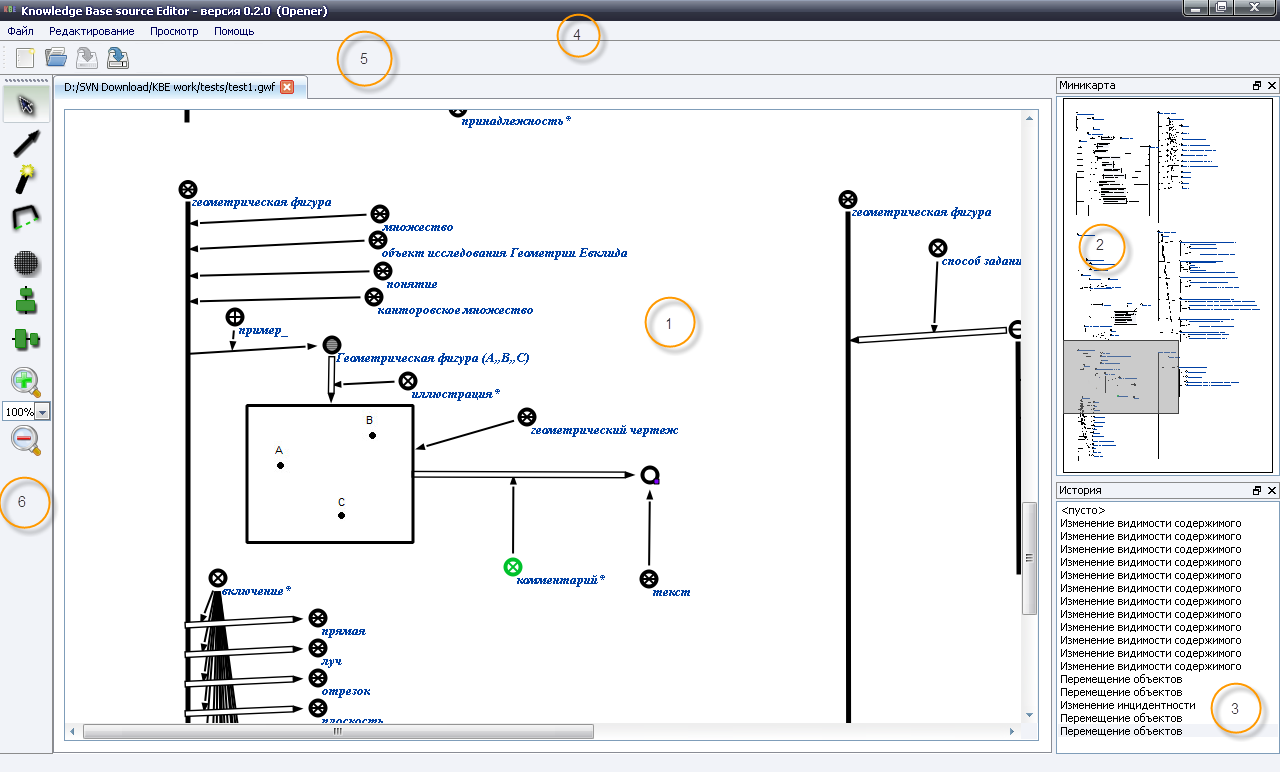
\includegraphics[width=16.23cm, height=9.82cm]{../images/mainwindow.png}
%	\caption{Главное окно приложения. 1 – основная рабочая область; 2 – миникарта; 3 – история внесенных в открытый документ 				изменений; 4 – строка меню; 5 – главная панель инструментов; 6 – панель sc.g-инструментов.}
%	\label{mainwindow}
%\end{figure}
%Главное окно приложения представляет собой некоторый набор вкладок и инструментов, которые легко можно перемещать, создавая свою собственную компоновку.

%\subsubsection{Основная рабочая область}

%Основная рабочая область предоставляет пользователю пространство, состоящее из нескольких вкладок, количество которых соответствует количеству открытых на текущий момент документов. Каждая вкладка является фрагментом исходных текстов базы знаний представленном на некотором внешнем языке. Описание основных действий с объектами рабочей области см. в разделе~\ref{usage}.

%\subsubsection{Миникарта и История изменений}

%Миникарта предназначена для легкой и быстрой навигации по открытому документу. История внесенных изменений позволяет пользователю отменять и возвращать действия, которые он произвел в ходе редактирования документа.

%\hrule\smallskip
%\noindent
\includegraphics[width=25pt, height=25pt]{../images/lamp.png} \textcolor[rgb]{.25, .67, .2}{\textbf{Примечание}: Если после отмены группы операций произвести какое либо действие, связанное с редактированием, то отмененные операции будут утеряны.}
%\smallskip
%\hrule

%\subsubsection{Строка меню}

%Строка меню содержит основные команды для работы с приложением.
%\begin{figure}[h]
%	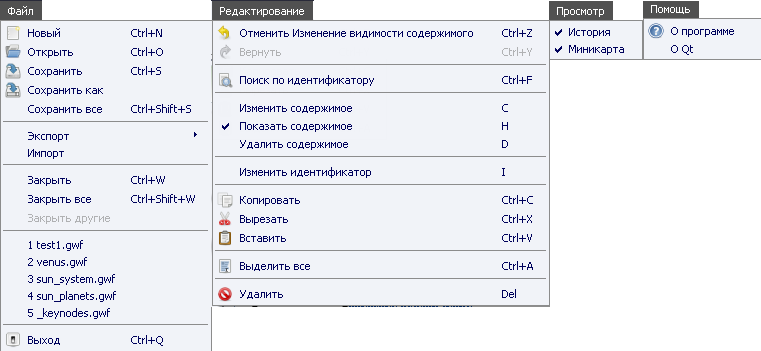
\includegraphics[width=16.22cm, height=7.51cm]{../images/menus.png}
%	\caption{Основные меню приложения.}
%	\label{menus}
%\end{figure}

%\hrule
%\smallskip
%\noindent
\includegraphics[width=25pt, height=25pt]{../images/lamp.png} \textcolor[rgb]{.25, .67, .2}{\textbf{Примечание}: Меню “\textbf{Редактирование}” будет содержать действия в зависимости от выделенных на данный момент объектов. Также оно частично дублируется контекстным меню объекта (открывается по нажатию правой клавищи мыши на объекте).}
%\smallskip
%\hrule

%\subsubsection{Главная панель инструментов}
%Содержит основные операции, необходимые для изменения состояния документа.
%\begin{figure}[h]
%	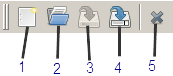
\includegraphics[width=5.72cm, height=2.57cm]{../images/maintoolbar.png}
%	\caption{Главная панель инструментов. 1 – создание нового документа; 2 – открытие уже существующего документа; 3 – сохранить 		текущий документ; 4 – сохранить текущий документ как…; 5 - закрыть текущую вкладку .}
%	\label{maintoolbar}
%\end{figure}*/
